\apendice{Plan de Proyecto Software}

\section{Introducción}

La intención de este anexo es la de dar a entender el plan de proyecto que se ha seguido a la hora de realizar este trabajo.

Primero se hablará sobre la planificación temporal seguida y más adelante su viabilidad tanto económica cómo legal

Las metodologías ágiles (especialmente Scrum) utilizadas en el desarrollo de este proyecto son aquellas que permiten ir adaptando la forma y carga de trabajo a medida que se desarrolla el proyecto, analizando los nuevos retos que pueden surgir durante la realización del mismo lo que otorga flexibilidad al proyecto durante la etapa de desarrollo.\cite{Hayat_2019}

\subsection{Scrum}

Scrum es un marco ligero que ayuda a las personas, equipos y organizaciones a generar valor a través de soluciones adaptables para problemas complejos.

\cite{ken_schwaber_scrum_2020}

En la figura \ref{fig:scrum} se puede ver una ilustración del proceso de Scrum

Está basado en el empirismo y emplea un enfoque iterativo e incremental para el desarrollo del producto minimizando riesgos ya que en el caso de un desastre simplemente habría que dar marcha atrás hasta la última versión estable.

Esta metodología tiene dos pilares clave, el equipo Scrum y los eventos.

\begin{figure}[!h]
    \centering
    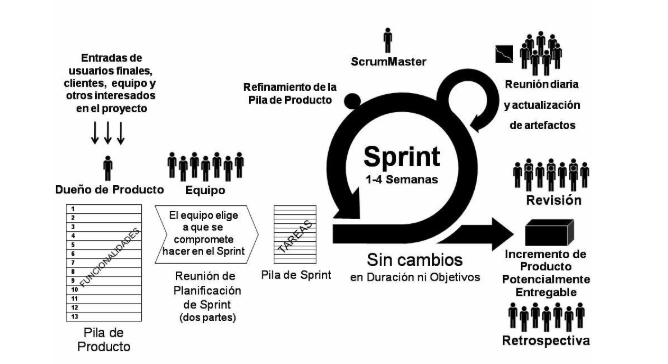
\includegraphics[width=1\textwidth]{img/Scrum.png}
    \caption{Ilustración del proceso de Scrum}
    \label{fig:scrum}
\end{figure}

\subsection{Equipo Scrum}

Capital humano que se encarga de desarrollar el proyecto. Constan de desarrolladores, product owner y Scrum Master.

\subsubsection{Desarrolladores}

Son los encargados de crear cada incremento al producto en cada sprint.

Sus tareas dentro del ciclo Scrum son la de crear un plan para el sprint llamado Sprint Backlog, Adaptar su plan de desarrollo día a día según los objetivos del sprint y responsabilizarse del trabajo de sus compañeros desarrolladores para garantizar un buen trabajo de todas las partes.

\subsubsection{Product owner}

El propietario del producto, es el responsable de sacar el máximo valor al trabajo del equipo Scrum así cómo gestionar la Backlog comunicando los objetivos a los que se desea llegar, se asegura de que se alcanza una buena calidad del producto final y gestionando los proyectos pendientes a realizar en el sprint.

\subsubsection{Scrum Master}

El máximo responsable de cumplir con la guía de Scrum, explicando cuidadosamente su teoría al resto del equipo así cómo coordinando su puesta en práctica.

Se responsabiliza de la efectividad del equipo Scrum eliminando las barreras entre los miembros, formándolos en la metodología y ayudándolos en sus planificaciones y tareas.


\subsection{Eventos de Scrum}

Los eventos en Scrum son oportunidades señaladas en el tiempo para revisar y adaptar los artefactos de Scrum, se crean para crear una regularidad y minimizar reuniones imprevistas.

\subsubsection{El Sprint}

Eventos de longitud fija donde ocurre todo el trabajo y en el que se fijan distintos objetivos.

En estos sprints iterativos se buscan realizar cambios que no deterioren el objetivo del sprint ni disminuya su calidad y clarificar los objetivos revaluando las tareas pendientes a medida que se desarrolla el proyecto.

\subsubsection{Planificación de Sprint}

Este evento inicia el Sprint estableciendo los objetivos a realizar en el mismo, este evento requiere de la participación del equipo de Scrum al completo.

Se pretende responder las siguientes cuestiones:

\begin{itemize}

    \item ¿Por qué este Sprint es valioso?
    \item ¿Qué se puede hacer este Sprint?
    \item ¿Cómo se realizará el trabajo elegido?

\end{itemize}

\subsubsection{Scrum diario}

Su propósito es el análisis del avance hacia el objetivo final del Sprint.
Es un evento de corta duración para los desarrolladores en los que discuten las diversas tareas del día.

\subsubsection{Revisión del Sprint}

Este evento que sucede al finalizar un Sprint tiene cómo propósito analizar este mismo, se revisan los logros conseguidos, los cambios que han tenido lugar y objetivos futuros.

\subsubsection{La retrospectiva del Sprint}

El objetivo de este último evento es el de aumentar la calidad del proyecto analizando el anterior sprint determinando que fue bien en el mismo, así cómo dificultades y la resolución o no de éstas.

Este evento concluye el Sprint

\subsection{Artefactos de Scrum}

Son la representación de los objetivos tanto a corto como a largo plazo del proyecto.

\subsubsection{Pila del producto}

Es una lista ordenada de lo que se necesita para mejorar el producto, los ítems en la pila del producto se consideran listos para su selección en un evento de planificación de Sprint.

\subsubsection{Pila del Sprint}

El trabajo pendiente por hacer en el Sprint. Se puede entender como el trabajo que aún le queda a los desarrolladores para alcanzar el objetivo de ese sprint.

\subsubsection{Incremento}

El incremento es cada pequeño objetivo cumplido que aporta un paso más hacia completar el objetivo del Sprint. Cada incremento es aditivo y deben funcionar todos juntos para llegar a la meta final. \cite{schwaber2020guia}


\section{Planificación temporal}

Para la realización de este trabajo se ha seguido la metodología Scrum mediante la aplicación de Zube.io lo que ha dado lugar a la Siguiente planificación mediante Sprints.

\subsubsection{Sprint 1: Sprint inicial}

En este primer Sprint se pretendía tener una toma de contacto inicial con las herramientas que se iban a desarrollar a lo largo del proyecto, en especial se asignaron dos objetivos principales, familiarizarse con el entorno de Zube así como investigar las tecnologías de RAG y de LLMs.

\ref{fig:sprintinicial}

\subsubsection{Sprint 2: Prueba de modelos}

Segundo Sprint del proyecto, el objetivo era investigar los diferentes modelos de LLM, sus respuestas ante datos clínicos y cómo implementarlos, así cómo sus formas de pago si lo requiriese.

\ref{fig:pruebamodelos}

\subsubsection{Sprint 3: Creación del primer modelo funcional}

En este Sprint se creó el primer chatbot funcional con la primera implementación del proceso de RAG con los datos finales sacados de PubMed. También se empezó con el desarrollo de la memoria.

\ref{fig:modelofuncional}

\subsubsection{Sprint 4: Mejoras}

En este pequeño Sprint se creó el repositorio en GitHub y se realizaron mejoras al código del modelo, eliminando código innecesario.

\ref{fig:mejoras}

\subsubsection{Sprint 5: Marco Teórico}

Este Sprint tenía cómo objetivo inicial la creación de una interfaz gráfica web en streamlit, lamentablemente aparecieron multitud de problemas con la GPU permitida y se decidió dejarla en la backlog list. Al final en este sprint se realizó el desarrollo del marco teórico de la memoria.

\ref{fig:teorico}

\subsubsection{Sprint 6: Finalización del Marco Teórico y actualización de Anexos}

En este Sprint se finaliza lo empezado en el anterior sprint y se empieza a trabajar en los anexos, sobre todo en el de Planificación y Datos así cómo se investigó el anexo de sostenibilidad.

\ref{fig:anexos}

\subsubsection{Sprint 7: Creación de la interfaz gráfica de usuario, validación del modelo y trabajo en los anexos}

El objetivo principal de este sprint fue el de acabar la herramienta añadiendo la interfaz gráfica de usuario, es decir la parte visual que comunicará al usuario con el software del programa para hacerlo más manejable gestionando las entradas y mostrando las salidas, además se empezó a trabajar en la validación del modelo, creando una escala numérica en la que el desarrollador, otros LLMs y personas ajenas al proyecto que cumplen el rol de futuros usuarios, dieron su opinión interactuando con el modelo y puntuandolo en dicha escala numérica. Mientras este trabajo se desarrollaba también se actualizaban los anexos de la documentación del proyecto.

\subsubsection{Sprint board}

\begin{figure}[h!]
    \centering
    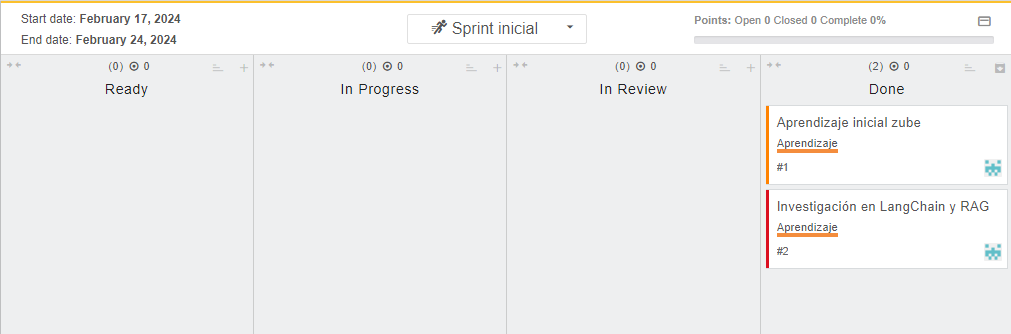
\includegraphics[width=1\textwidth]{img/SprintInicial.png}
    \caption{Sprint Inicial}
    \label{fig:sprintinicial}
\end{figure}

\begin{figure}[h!]
    \centering
    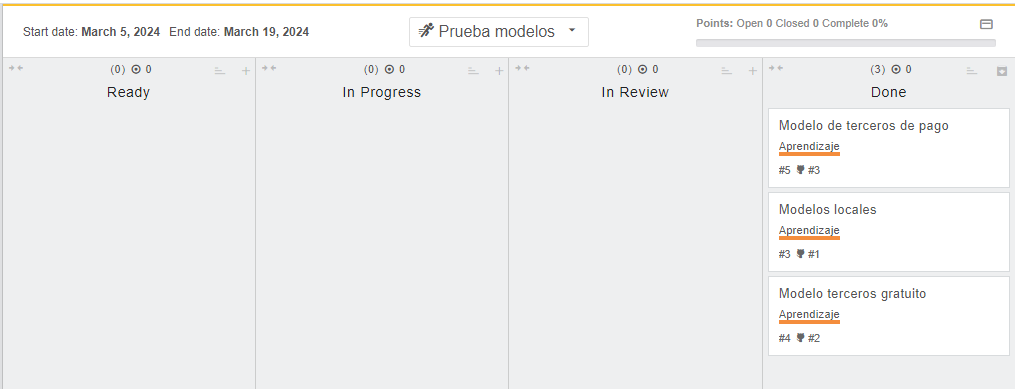
\includegraphics[width=1\textwidth]{img/PruebaModelos.png}
    \caption{Sprint Prueba Modelos}
    \label{fig:pruebamodelos}
\end{figure}

\begin{figure}[h!]
    \centering
    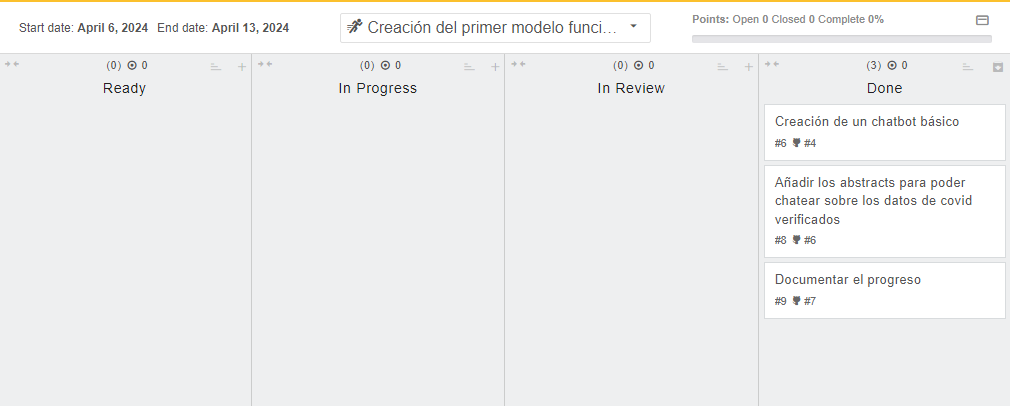
\includegraphics[width=1\textwidth]{img/modelofuncional.png}
    \caption{Sprint creación del primer modelo funcional}
    \label{fig:modelofuncional}
\end{figure}

\begin{figure}[h!]
    \centering
    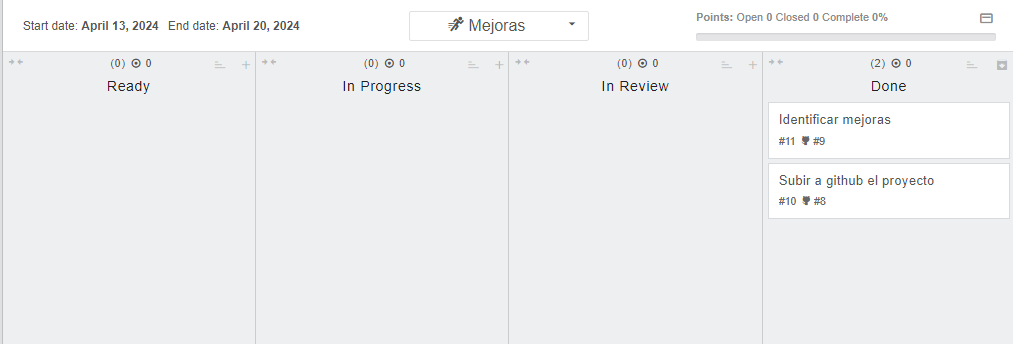
\includegraphics[width=1\textwidth]{img/Mejoras.png}
    \caption{Sprint Mejoras}
    \label{fig:mejoras}
\end{figure}

\begin{figure}[h!]
    \centering
    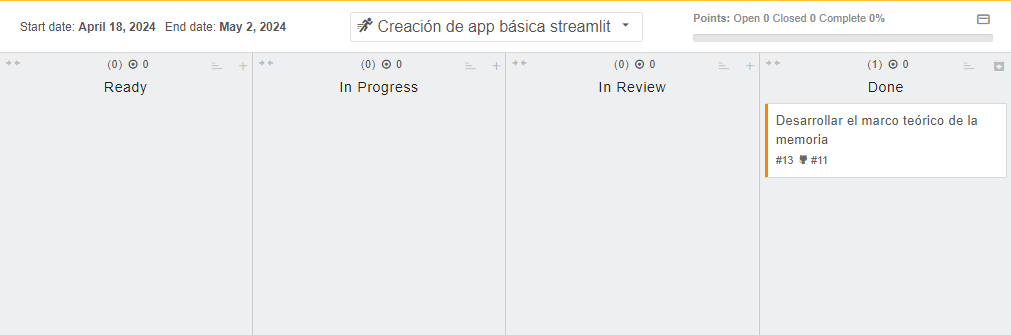
\includegraphics[width=1\textwidth]{img/teorico.png}
    \caption{Sprint Marco Teórico}
    \label{fig:teorico}
\end{figure}

\begin{figure}[h!]
    \centering
    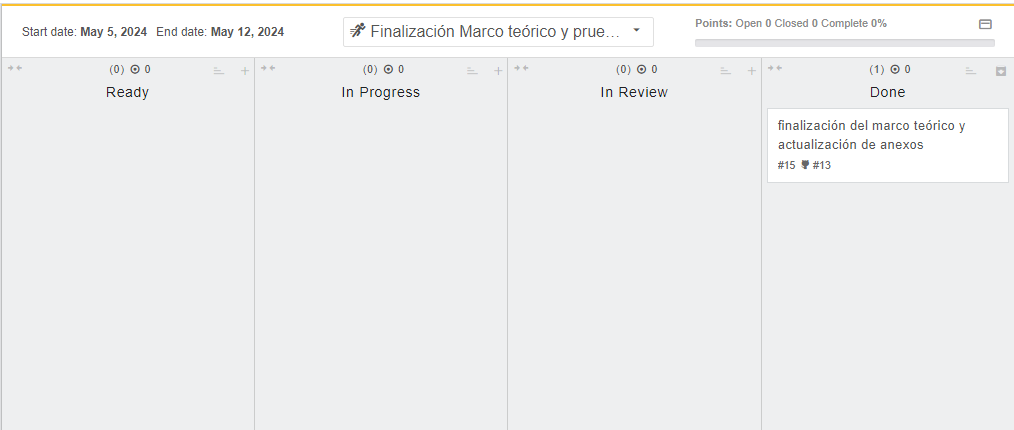
\includegraphics[width=1\textwidth]{img/anexos.png}
    \caption{Sprint Anexos}
    \label{fig:anexos}
\end{figure}

\begin{figure}[h!]
    \centering
    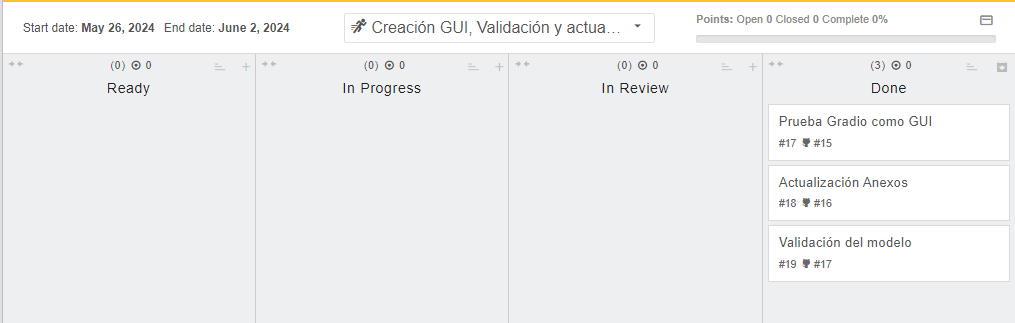
\includegraphics[width=1\textwidth]{img/gui.png}
    \caption{Sprint GUI}
    \label{fig:gui}
\end{figure}

\FloatBarrier

%TODO ir acabando los sprints a medida que los acabe

\subsection{Planificación económica}

En este apartado se analizarán los costes monetarios de la implementación del proyecto

\subsubsection{Librerías}
%TODO De momento todo lo empleado es de código abierto pero podría cambiar

Las librerías empleadas en el desarrollo han sido de código abierto por lo que no suman ningún coste.

\subsubsection{Contratación}

Se estima que el sueldo promedio de un programador Junior en España sería de 1750 euros brutos al mes a la fecha de realización de este proyecto como indica en la figura \ref{fig:Salario}, asumiendo que los pluses y complementos así cómo la parte proporcional de las pagas extra está incluida. \cite{talent_salario_2024} 

\begin{figure}[h!]
    \centering
    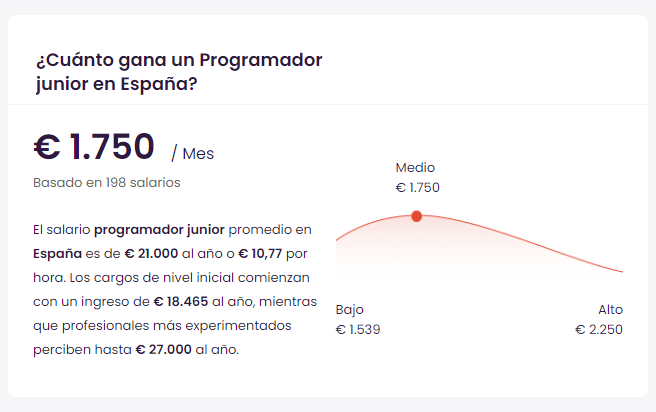
\includegraphics[width=1\textwidth]{img/Salario.png}
    \caption{Salario de un Programador Junior en España}
    \label{fig:Salario}
\end{figure}

También asumimos de manera arbitraria ya que esto cambiará dependiendo de multitud de condiciones un 9\% de Retención de IRPF y unas cotizaciones, enfermedad profesional y accidentes de trabajo del 35\%.

El resultado del cálculo sería una base de cotización de 1750 euros a los que se le tendrán que sumar los costes de la seguridad social que ascienden hasta los 525 (0,3*1750) euros calculados teniendo en cuenta lo siguiente:

\begin{itemize}

    \item 23.60\% contingencias comunes
    \item 5.5\% tipo general de desempleo para un contrato indefinido
    \item 0,20\% FOGASA (Fondo de Garantía Salarial)
    \item 0,70\% formación profesional

\end{itemize}

El coste de contratar a un programador junior al mes asciende a los 1750 euros + 525 euros = 2275 euros al mes. Si la duración del proyecto ha sido de 3 meses, el coste total de mano de obra es de 2275 euros * 3 meses = 6825 euros. \cite{Billin_2014}

\subsubsection{Web}

Si se quisiera desplegar la aplicación Gradio ofrece hosting a través de los spaces de Hugging Face que puede ser gratuito o de pago. Teniendo en cuenta la GPU necesaria para ejecutar los modelos, sería conveniente emplear las opciones de pago que facilitan la aceleración de GPU, Hugging Face ofrece el espacio NVidia T4 small * 4vCPU * 15GB por 0,40 Dólares la hora, declarándose "dormidos" tras una hora de inactividad, este tiempo no se cobra.

\cite{Hugging_Face_2016}

\subsection{Amortización de equipos}

El valor total de adquisición de los equipos informáticos utilizados es de XXX euros. Suponiendo un periodo de amortización de 5 años, los costes de amortización para la duración de este proyecto de 3 meses son (XXX/5)*(3/12) = YYY

\subsection{Viabilidad legal}
\subsubsection{Licencias}
Las librerías empleadas son Open Source.

Las licencias de las librerías empleadas son las siguientes:

\begin{itemize}

    \item Licencia de Python Software Foundation
    \item Licencia BSD modificada
    \item Licencia Apache 2.0
    \item Licencia MIT

\end{itemize}

El código publicado en el repositorio está licenciado con licencia MIT.

\subsubsection{Legislación}

Según la Ley de inteligencia artificial publicada el 13 de marzo de 2024 las inteligencias artificiales se pueden clasificar en cuatro grupos según su riesgo:

\begin{itemize}

    \item Riesgo inaceptable
    \item Riesgo alto
    \item Riesgo limitado
    \item Riesgo mínimo o nulo

\end{itemize}

Cuando una inteligencia artificial presente una clara amenaza para la seguridad y/o los derechos de las personas estas estarán catalogadas cómo de riesgo inaceptable y, por lo tanto, prohibidas.

Las IAs que se empleen en infraestructuras críticas, formación profesional, componentes de seguridad, gestión de empleo, servicios públicos y privados esenciales, administración de justicia o gestión de la migración serán considerados de alto riesgo.

Estas IAs estarán sujetas a estrictas regulaciones cómo, exhaustivos controles de calidad, registros de actividad constantes y medidas adecuadas de supervisión humana.

Los riesgos limitados incluyen a los que puedan presentar problemas relacionados a la falta de transparencia en el uso de las mismas. Por ello sólo se permitirán aquellas IAs de Riesgo limitado las cuales aporten la suficiente información a su usuario.
Un ejemplo de esto sería un chatbot que sólo estaría permitido en el caso de que no hubiese ninguna en la interacción hombre-máquina, es decir, que el usuario siempre sea consciente que no está chateando con una persona real.

Las IAs de riesgo nulo cómo los filtros de spam o las usadas en videojuegos no tienen restricciones.

El proyecto cumple con la Ley de inteligencia artificial ya que se trata de una inteligencia artificial de Riesgo limitado en la que los usuarios en todo momento conocen que están interactuando con una máquina.\cite{CE_ley_2024} 

Para entender la viabilidad legal de los datos hay que consultar su fuente original, PubMed, los artículos ahí publicados son recursos gratuitos que apoyan la investigación y recuperación de literatura biomédica.\cite{Anandhu_H_abstracts_2023}

